La conversione di documenti in un formato strutturato avviene abilitando il server GROBID. Per avviare il servizio, è possibile usufruire di alcune \textbf{immagini Docker} preconfigurate oppure installare integralmente il software tramite \textbf{Gradle}, anche se questa opzione richiede una previa installazione di una JDK. Una volta attivato, il server sarà raggiungibile alla porta $8070$ del dispositivo, consentendo di verificare il corretto funzionamento della libreria. \vspace{7pt} \\
Dal punto di vista implementativo, è stata adottata la prima soluzione, in cui Docker ha garantito un'elevata facilità di deployment e ha permesso di utilizzare i modelli di machine learning senza importare alcuna dipendenza software. \vspace{7pt} \\
Il team di sviluppo ha fornito due immagini Docker, le quali differiscono in base all'accuratezza della trasformazione e alla velocità di computazione. A tal proposito, è stata preferita l'impostazione più leggera, sacrificando parte della precisione per ottenere tempi di elaborazione più rapidi: sul computer in cui il codice è stato eseguito, la conversione dei file ha richiesto poco più quattro ore.
\begin{lstlisting}[language=python, caption=Conversione di documenti PDF in file XML/TEI]
from grobid_client.grobid_client import GrobidClient

try:
    grobid_client = GrobidClient(config_path="../config.json")
    grobid_client.process(
        "processFulltextDocument",
        input_dir,
        output_dir,
        n=10
    )        
except requests.exceptions.ConnectionError as e:
    print("Connection error during Grobid processing: ", e)
except Exception as e:
    print("Error during Grobid processing: ", e)\end{lstlisting}
Il codice illustra il processo di trasformazione dei documenti, memorizzati all'interno di una determinata cartella. Il passaggio iniziale consiste nella creazione di un \textbf{client} in grado interagire con il servizio abilitato e di stabilire il momento in cui debba essere avviata la conversione. \vspace{7pt} \\
Prima di procedere, occorre sottolineare l'importanza del file JSON dato in ingresso all'istanza della classe \textbf{GrobidClient}. Il file di configurazione possiede alcune proprietà personalizzabili, sintetizzate in:
\begin{itemize}
    \renewcommand{\labelitemi}{-}
    \item \textbf{grobid\_server}: indica il Uniform Resource Locator dove il server sarà raggiungibile.
    \item \textbf{batch\_size}: descrive la dimensione del thread pool impiegato dal \textbf{ThreadPoolExecutor}, determinando il numero massimo di flussi di esecuzione gestiti internamente. La documentazione consiglia di non variare il valore di default, dato che rappresenta un numero sufficientemente alto per garantire un'elaborazione efficiente, ma non eccessivo, in modo tale che sia preservata la memoria della macchina.
    \item \textbf{sleep\_time}: definisce il tempo di attesa prima di inviare una nuova richiesta a GROBID quando il server segnala che tutti i suoi thread sono attualmente occupati. Il tempo di attesa varia a seconda alla tipologia di conversione: nel caso in cui il documento sia convertito nella sua interezza, noto come \textbf{proccessFullTextDocument}, è consigliato un intervallo di 5-10 secondi, mentre per attività di \textbf{processHeaderDocument} è sufficiente un tempo di attesa pari a 2 secondi.
\end{itemize}
Al termine della conversione, il risultato restituito consiste in un insieme di risorse di estensione \textbf{XML/TEI}. I pattern ripetitivi dei tag XML hanno facilitato l'estrapolazione delle informazioni desiderate, utilizzando la libreria \textbf{BeatifulSoup}. \vspace{7pt} \\
Il package è progettato per analizzare contenuti basati su linguaggi di markup, organizzandoli in una struttura dati ad albero. Questo permette di accedere agevolmente alle differenti entità che compongano un articolo scientifico, ognuna delle quali dispone di propri parametri, a seconda degli attributi e del corpo dell'elemento.
\begin{figure}[H]
    \centering
    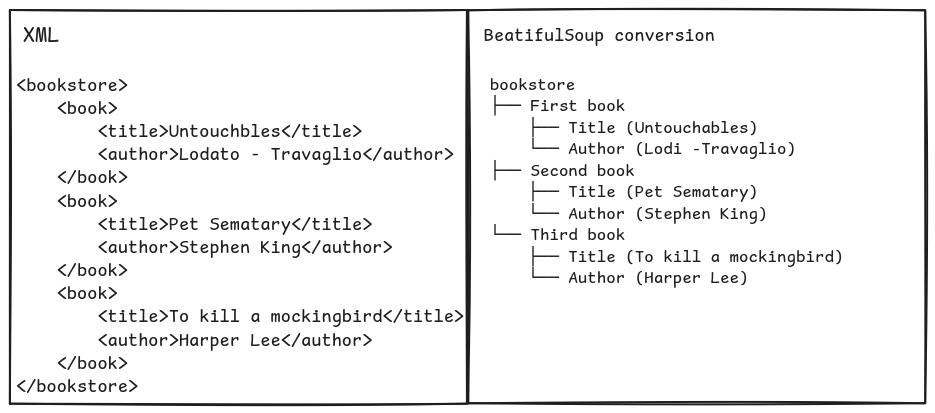
\includegraphics[width=.7\textwidth]{img/img4.png}
    \caption{Organizzazione dei tag XML secondo una struttura ad albero}
    \label{fig:3.2.1-3.1}
\end{figure}
Di seguito è definito lo snippet di codice che si avvale di BeatifulSoup per ricavare i metadati necessari. Qualora non vi sia corrispondenza tra la struttura dati e la lista di tag XML data in ingresso, è restituito un valore \textbf{None}.
\begin{lstlisting}[language=python, caption=Estrazione dell'informazioni tramite BeatifulSoup]
from bs4 import BeautifulSoup

def extract_content(soup: BeautifulSoup, tags: List[str]) -> str:
    try:
        element = soup.find(tags[0])

        for tag in tags[1:]:
            element = element.find(tag)

        return element.contents[0]
    except Exception:
        return None\end{lstlisting}
Le informazioni ricavate sono inserite iterativamente all'interno di una lista di oggetti di tipo \textbf{Metadata} (\ref{lst:Metadata}), per poi essere adoperate durante la fase di acquisizione dei riferimenti bibliografici.